\documentclass[a4paper,12pt]{report}
\usepackage[utf8]{inputenc}

\usepackage[unicode,colorlinks,linkcolor=blue,urlcolor=blue]{hyperref}

\PassOptionsToPackage{defaults=hu-min}{magyar.ldf}

\usepackage[magyar]{babel}
\usepackage{graphicx}
\usepackage{textgreek}
\usepackage[delims]{lgreek}
\usepackage{couriers}
\usepackage{amssymb}

\usepackage{amsfonts}
\usepackage{amssymb}
\usepackage{graphicx}
\usepackage{titlesec}
\usepackage{booktabs}
\usepackage{multicol}

\usepackage[top=25mm, bottom=25mm, left=35mm, right=25mm]{geometry}

\usepackage{setspace}
%\usepackage{listings}

\titleformat{\chapter}{\normalfont\huge}{\thechapter.}{20pt}{\huge}


\sloppy
\linespread{1.5}
	
\begin{document}

\tableofcontents

\chapter{Bevezetés}
A szoftverfejlesztési folyamatban egyre nagyobb hangsúlyt kap a tervezés, a rendszer strukturálása a felelősségi körök szeparálásnak elve, az újrafelhasználhatóság, valamint a rendszer szereplőinek izoláltsága szerint. Az UML \cite{uml_omg}, ezen belül is a végrehjatjható UML ezen a ponton játszik nagy szerepet, melynek segítségével magas szinten leírhatjuk a rendszer struktúráját, felvehetjük az egyes szereplőket úgy, hogy már a rendszertervünk is tesztelhetővé, a kódgenerálás révén pedig közvetlen felhasználhatóvá válik. \\ A szereplők izolálása érdekében kommunikációs csomópontokra, portokra és azokat összekapcsoló absztrakt kommunikációs protokollokra, konnektorokra van szükségünk, melynek révén az adott szereplőnek nem szükséges ismernie a kommunikációban részt vevő felet. Valós idejű rendszerek tervezésnél fontos szerepet játszanak a portok és konnektorok \cite{uml_real}\\ 
A portok és konnektorok fordíthatóságához meg kell ismerni azok pontos UML szemantikáját,a szabvány szerinti reprezentációját, valamint kell találni egy olyan C++ reprezentációt, melynek API-ja letisztult, érhető a felhasználó számára, ugyanakkor az egyes műveletek leghatékonyabb megvalósítására törekszik. A következőkben ezeket a megvalósításokat fogjuk elemezni, egymással összehasonlítani, valamint kiérünk a szabványos UML leképezésre, annak problémáira is. 

\section{UML Komponens fogalmak}
\subsection{Enkapszulált elem}
UML-ben az enkapszulált elem egy olyan abstrakt fogalom, egyfajta mechanizmust fejez ki, mellyel képesek vagyunk elszigetelni az objektumot a külvilágtól portok segítségével.\\ Ez a fogalom nem összekeverendő az UML komponenssel, mely egy enkapszulált elem, viszont több klasszifikált elemet fog össze, egy jól definiált interfésszel rendelkezik, mellyel valamilyen szolgáltatást nyújt a külvilág felé. A komponens fontos tulajdonsága, hogy az adott rendszerben könnyen cserélhető. \\
Az UML Osztályok is enkapszulált klasszifikációnak számítanak, a diplomamunka az osztályok portjainak exportálását járja körül.
\subsection{UML Interfész}
UML-ben az interfész egy olyan klasszifikáció, melynek a szokványos operációs műveleteken kívül speciális kommunikációs műveletei, úgynevezett reception-ei vannak. Ezek olyan speciális műveletek, melyek egy eseményt várnak, tehát egy interfész leírja, milyen eseményekkel kommunikálhatunk az interfészeken keresztül.
\subsection{UML Port}
Enkapszulált elemek egy adattagja, amely egy kommunikációs csomópontot reprezentál. A típusa lehet egy egyszerű primitív is, de gyakoribb eset, amikor a port egy interfészt valósít meg. Ilyen esetben megkülönböztetünk szolgáltatott és elvárt interfészeket. A szolgáltatott interfész a külvilágtól érkező üzenteteket foglalja magában, míg az elvárt interfész a külvilággal történő kommunikációra szolgál. Arra használjuk, hogy egy klasszifikációt függetlenítsünk a környezetétől, mivel így a külvilággal való kapcsolattartás egy bizonyos típusú porton keresztül történik, nem pedig referencia birtoklásával.
\subsection{UML Connector}
Egy asszociációt realizál két port között. Leírja, hogy milyen portokat köt össze, assembly vagyd delegáció kapcsolat van-e két port között, illetve a kommunikációra használt protokollt.

\chapter{Áttekintés}

\section{A probléma rövid meghatározása}
A diplomamunka célja teljes körű támogatást nyújtani az interfész portokkal történő kommunikációra a txtUML keretrendszeren belül. A portokat és azok műveleteit az eszköz által helyesen és teljesen leírhatónak tekintjük, ennek problémájával nem foglalkozunk. A probléma megtalálni ennek a helyes UML reprezentációját, mellyel a kódgenerálás tovább tud dolgozni, valamint a megfelelő C++ kód reprezentációt, mely megfelelő hatékonyságú és tisztaságú.

\section{Szabványok és keretrendszerek áttekintése}
\subsection{fUML - ALF}
A Foundational UML (fUML) \cite{fmul} egy Object Managment Group (OMG) által specifikált végrehajtató UML szabvány, 
melynek szöveges akciónyelvi szintaxisát az ALF (Action Language for Foundational UML) \cite{alf} definiálja.
Mivel ALF az UML szabvány egy részhalmazán alapszik, így az akciónyelvi elemekhez és a strukturális elemekhez (osztály, asszociációk)  széleskörű támogatást nyújt, de az állapotgépekhez vagy a kompozíciókhoz nem definiál szintaxist.

\subsection{Umple}
Az Umple \cite{umple} szöveges alapú modellezőeszköz támogatja a komponens struktúrák leírását. Itt a portok egyszerű adattagonként jelennek meg, melyekhez úgynevezett aktívator metódusokat rendelhetünk, melynek hatása az attribútum változásakor érvényesül. A megváltozott érték pedig végig csorog a kapcsolatban álló portokon, melyre szintén egy aktivátorok segítségével reagálhatunk. A konnektorok pedig egyszerűen portok egymáshoz kötésével jelennek meg (binding) konnektor struktúrák és interfész kompatibilitási problémák nélkül. Ezzel szemben a \textit{txtUML}-ben interfész portokat adhatunk meg elvárt és szolgáltatott interfésszel, egyszerű attribútumokat nem, aktivátorok helyett pedig az állapotgép átmenteti vannak kiegészítve a portok dimenziójával. Az Umple nem foglalkozik a szabványos UML2-es reprezentációval, a C++ kódot közvetlen a modell szövege alapján állítja elő. Valamint saját akciónyelvvel sem rendelkezik, hanem azt a célnyelvben adhatjuk meg. \\

Előnyei:
\begin{itemize}
\item Online eszközként is elérhető, nem szükséges hozzá semmit telepíteni.
\item Letisztult, jól definiált szöveges szintaxisa van, beleértve a portokat is.
\item Tartalmaz kódgenerálást
\end{itemize}
Hátrányai:
\begin{itemize}
\item Nem generál egy szabványos UML modellt a kódgenerálás előtt, közvetlen a szövegre építkezik.
\item A portokat egyszerű adattagként képzi le a feltípusozás alapján, nem lehet megadni szolgáltatott és elvárt interfészeket.
\item Nincs saját akciónyelve
\item Nincs lehetőség testre szabni az üzenetküldés implementációját a porton keresztül, nincs konfigurációs leírás
\end{itemize}

\subsection{StartUML}
A StartUML  Támogatja a kompozit diagramok létrehozását, így a portok, konnektorok és interfészekét is. Vizuális modellezőeszköz, a létrehozott diagramokból C++ kódot tudunk exportálni. A Portok vázát exportálja, ahogy az interfészeket is, de primitív szinten, a portok féltípusozása után egy adattagként generálja hozzá az osztályhoz. A konnektorokat már nem exportálja, ahogy a portokhoz kapcsolódó műveleteket sem. \\
Előnyei:
\begin{itemize}
\item Az UML szabványos elemeivel dolgozik
\item Különböző kiterjesztések révén tartalmaz kódgenerálást
\end{itemize}
Hátrányai:
\begin{itemize}
\item Az eszköz mellett meg kell ismerni precízen az UML szabványos elemeit is, hogy fel tudjuk tölteni az elemek tulajdonságait
\item A kódgenerálás csak a vázra terjed ki, mely tartalmazza a portoka, de az azokkal való műveleteket már nem.
\item Nehézkes, vizuális használat, az elemeket szabadon létrehozhatjuk, és könnyen nem szabványos modellt generálhatunk, míg a txtUML exportja a szabványos modellt exportálás révén hozza létre, így kisebb lehetőségünk van hibázni.
\end{itemize}

\subsection{BrigePoint UML}
A StartUML-hez hasonlóan az UML szabványos elemeiből építhetünk fel vizuálisan egy szabványos UML diagramot. Azonban nem tudunk osztályok között portokkal kommunikálni, csak a komponensek között, így ez a megoldás nem elég általános. Portot, illetve konnektort önmagában nem tudunk felvenni, az interfészek segítségével tudunk egy kapcsolatot húzni két komponens között, mely leképződik egy porttá és konnektorrá. Hasonlóan a StartUML-hez, az akciókat aktivitás node-ok révén kézzel kell összerakni, így nehéz szabványos port műveleteket létrehozni. Összességében a BridgePoint-ról \cite{bridge} is elmondható, hogy kezdetlegesen támogatja a portokkal történő kommunikációt, de kiforratlan, hiányos, a kódgenerálás ellenére nehéz érdemben azok reprezentációjáról beszélni. 

\section{Összefoglalás}
Összességében az figyelhető meg az egyes exportálási módok között, hogy a portokat mindig valamilyen primitív feltípusozott adattagként exportáljuk. A másik lehetőségünk, melyet mi is követni fogunk, az interfész portokat összetett típusként exportálni, melyben benne van a szolgáltatott és elvárt interfészt. Portok összekapcsolásának, a portokon történő kommunikáció végrehajtási szemantikájával pedig nem mindegyik keretrendszer foglalkozik, még ha részben támogatja is a portok exportálását. Ennek oka a szabvány nehezen érthetőségében és hiányosságában keresendő. Mindebből az figyelhető meg, hogy egy viszonylag új területről beszélünk, melyben egy teljesen körű támogatás és elemzés referencia értékű lehet későbbi megoldások, fejlesztések számára. A diplomamunka kielemez több különböző, teljes körű támogatást a portok és interfészek C++ nyelvre történő exportáláshoz, mely magában foglalja a szabványos UML modell létrehozását egy jól definiált leírónyelv alapján.

\chapter{Reprezentációs lehetőségek}
\section{A megfelelő reprezentációk megtalálása}
Az eddig leírtakból kiderült, hogy a szabványos reprezentáció megtalálásával is problémákba ütközünk, mely a fellelhető irodalomból és eszközökből is csak nehezen derül ki, így kitérünk ezek ismertetésére is. A C++ reprezentációhoz pedig egy saját Port könyvtárat és generálási módszert választunk, mely a felellethető módszerek finomításából és több különböző ötlet elemzésének következtében hozunk létre. \\

A továbbiakban a következő elemek reprezentációjával foglalkozunk:
\begin{itemize}
\item Interfészek
\item Portok és üzenet küldés/fogadás művelet
\item Konnektorok és connect művelet
\end{itemize}

\section{Portok reprezentálása}

\subsection{UML-ben}
A portok reprezentálása értelemszerű, egy speciális Property-t kell felvenni az osztályon belül. Amit fontos megemlíteni, hogy a szolgáltatott interfész segítségével fogjuk feltípusozni. 


\subsubsection{Szemléltetés osztálydiagrammal}
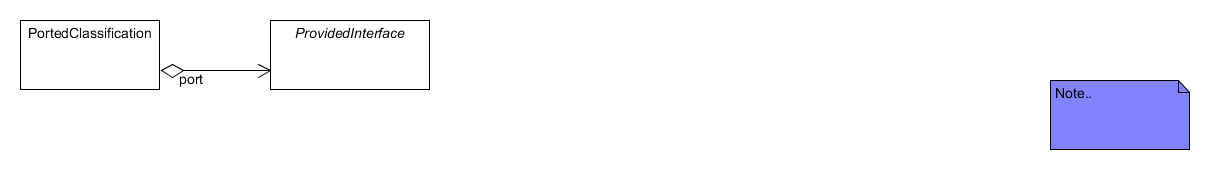
\includegraphics[scale=0.7]{uml_port_class.png}

\subsubsection{Szemléltetés komponens diagrammal}
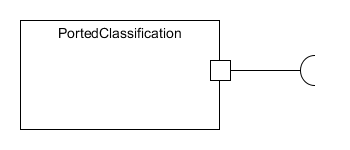
\includegraphics[scale=0.7]{uml_port_comp.png}

\subsection{C++-ban}
A portokat minden esetben adattagként reprezentáljuk, ezt mi sem tudjuk másképp megtenni. Többféle képen használhatók kommunikációra, de minden esetben egyfajta ravaszként működik a rajtuk történő állapotváltozás. A port adattag értéke reprezentálja az üzentet. Ennek megfelelően általánosságban kétféle megoldás létezik a portokon történő kommunikációra:
\begin{itemize}
\item Hasonlóan az események feldolgozásához, úgy a portokon történű üzenetáramlást is átmeneti függvényekkel dolgozzuk fel.
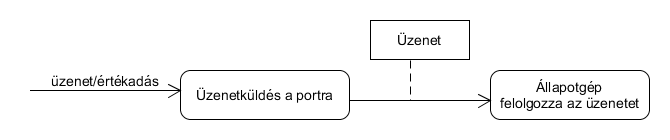
\includegraphics[scale=0.6]{port_actfun.png}
\item Külön aktivátor függvényeket valósítunk meg az osztályon belül az egyes portokra, melyek a portok állapotváltozások aktiválódnak. 
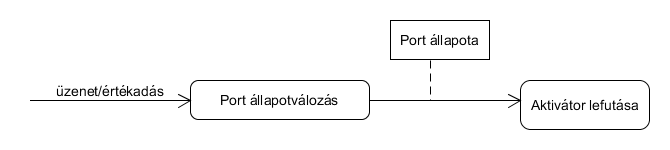
\includegraphics[scale=0.6]{port_sendm.png} \\
\end{itemize}

A mi esetünkben az előbbi megoldás tűnt kézenfekvőnek, mivel az könnyen adaptálható a meglévő generálási szabályok közé, valamint a forrásnyelv is ezt a konvenciót követi. 

\section{Portokra való üzenetküldés/fogadás reprezentálása} \label{message}
\subsection{UML-ben}
\subsubsection{Üzenet küldés}
A  \textit{SendObjectAction} két paraméterből áll, egy célobjektumból és egy üzenetből.
A célobjektum valamilyen \textit{InputPin}, vagyis valamilyen akciónak az eredménye.
Mivel a port egy strukturális elem, így a referenciáját egy \textit{ReadStructuralFeatureAction}-nal megszerezhetjük. 
\begin{itemize}
\item Könnyű reprezentálni, illeszkedik a modellfordító elvébe, aki feltételezi, hogy
egy \textit{send} akciónak van egy cél objektuma, ahova az üzentet kell küldeni.
\item Nem kell extra logikát beiktatni a C++ fordítóba az üzenetküldés terén.
\end{itemize}

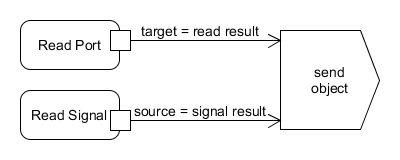
\includegraphics[scale=0.8]{send_uml.png}

\subsubsection{Üzenet fogadás}
Ha egy objektumnak a portján keresztül szeretnénk üzenetet küldeni a külvilág felől, akkor a \textit{SendObjectAction}-nak a az \textit{OnPort} műveletét használhatjuk. 

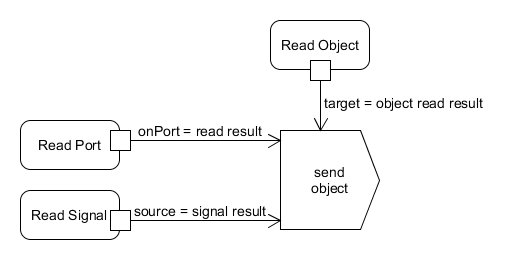
\includegraphics[scale=0.6]{receive_uml.png}

\subsection{C++-ban}
\subsubsection{Üzenet küldés}
Ez esetben már a \textit{send} művelet végrehajtási szemantikája érdemes számunkra. A \textit{send} művelet azt jelenti, hogy a Portra teszünk egy üzenetet, melyet továbbítunk egy másik komponens felé konnektoron keresztül. Ennek szemantikájával a \ref{connect} fejezetben majd foglalkozunk részletesen.

\subsubsection{Üzenet fogadás}
Valahogyan ki kell fejeznünk azt is, ha egy üzenetet nem a külvilág felé delegálunk, hanem a külvilág felől érkezett egy üzenet a Portra, melyet fel kell dolgoznunk állapotgéppel összekapcsolt portok esetén, vagy tovább delegálunk a belső komponensek felé. Erre két lehetősünk van: Vagy egy teljesen új függvényt vezetünk be (nevezzük ezt \textit{receive}-nek), vagy paraméterezzük a \textit{send} függvényünket. Előbbi megoldás tisztább, jobban érhető a felhasználó számára, valamint a szolgáltatott és elvárt interfészek kifejezésénél is előnyösebb lesz. (\ref{inf}) \\

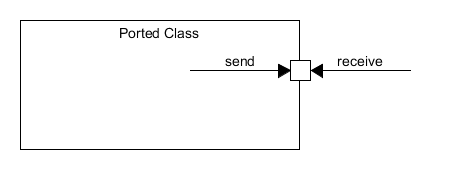
\includegraphics[scale=0.8]{send_rec.png}

\section{Interfészek reprezentálása interfész portok esetén} \label{inf}
\subsection{UML-ben}
Az interfészeket UML-ben értelemszerűen reprezentáljuk, annyiban különböznek csak az osztályoktól, hogy megadhatunk neki. fogadási műveleteket, un. receptionöket.

\subsection{C++-ban}
C++-ban számos lehetőségünk van kifejezni egy UML interfészt.
\subsubsection{Nincs interfész}
Egy lehetséges megoldás az is, ha nem vesszük figyelembe a szolgáltatott és elvárt interfészeket akkor, mikor egy adott portot manipulálunk, üzenetet küldünk rá. A forrásnyelv validációja hivatott kiszűrni az ilyen nem helyes üzenetküldéseket, hivatkozásokat. \\
Előnyök:
\begin{itemize}
\item Kódgenerálás szempontjából nagyon triviális megoldás, nem szükséges foglalkozni egyáltalán vele.
\item Alacsony szintű, hatékonysági kérdésekben a legjobb megoldás. 
\end{itemize}
Hátrányok:
\begin{itemize}
\item Külső komponensek, portok esetén magunk sem tudunk felvenni interfészeket, ilyenkor már nem hagyatkozhatunk a forrásnyelv validációjára, könnyen hibázhatunk.
\item Ha nem is vezetünk be új komponenst, külső kommutáció esetén tetszőleges üzentet küldhetünk a portra, ami szintén hibás lehet.
\item A generált kód kevésbé lesz érthető
\item Az interfészeket sehol máshol sem tudjuk felhasználni, osztályok esetén sem, mely szintén a modellel való kommunikációban jelent hátrányt. 
\end{itemize}

\subsubsection{Van interfész}
Ezen belül meg kell vizsgálni az interfész port szintaxisát, valamint a mögöttes végrehajtási szemantikát,illetve magának az interfésznek a leírási módjait. \\
Ahogy azt korábban írtuk, a port típusa az UML-ben a szolgáltatott interfész, ezért kézenfekvő megoldás lenne felvenni egy olyan adattagot, melynek ez az interfész a típusa. Ennek azonban több hátránya is van, sokkal nehezebben tudjuk kifejezni, milyen elvárt interfésze van a portnak, valamint nem tudjuk kifejezni a port típuson belül az üzenetküldés végrehajtási szemantikáját, valamilyen külső implementációra kényszerülünk. Ezáltal bonyolultjuk a megvalósítást, veszítünk az absztrakcióból, de a hatékonyságot nem növeljük. \\
Így a másik lehetőségünk bevezetni a Port típust, melynek sablon paramétere a szolgáltatott és elvárt interfész. Ezáltal a következőképpen vehetünk fel egy portot egy osztályba: \\


%\lstinputlisting[language=C++]{port_decl.h}

Ezek után technikailag többféle lehetőségünk van megvalósítani a validációt: \\
\begin{enumerate}

\item Generáljunk egy üres osztályt az interfészekből, majd a szignálok származzanak le aszerint, hogy melyik interfész fogadó műveletei között vannak benne: \\
PL: UML interfész neve: PingPongInterfce, a receptionjai pedig a következő szignálokat fogadják: Ping, Pong \\
Majd a portnak legyen egy \textit{send} művelete, ami az elvárt interfész alá sorolt szignálokat várja, vagyis olyan szignálokat, melyek implementálják a megfelelő interfészt.
Mindezzel fordítási időben biztosítjuk, hogy ne adhassunk át olyan szignált, melyet nem soroltunk az elvárt interfész szignáljai közé. Hasonlóan, a \textit{receive} művelet olyan szignálokat vár, melyek leszármazottjai a szolgáltatott interfésznek. \\

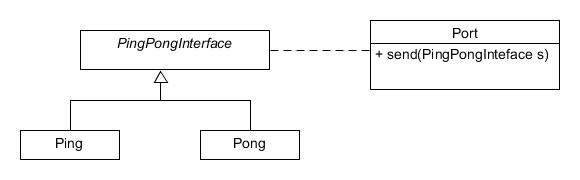
\includegraphics[scale=0.7]{inf_ver1.png} \\

Előnyök:
\begin{itemize}
\item Egyszerű megvalósítás, kevés extra kód generálásra van szükség hozzá, az interfészek lényegében csak üres, jelző osztályok
\item Egyetlen \textit{send} függvénnyel meg lehet oldani a validációt, így a kód a lehető legkisebb lesz, nem lesz technikai redundancia
\end{itemize}
Hátrányok:
\begin{itemize}
\item Nem általánosított megoldás. Az interfészt bármilyen szereplő használhat, és le is származhat belőle, azonban ezzel erősen portokra korlátozzuk a megoldást, mivel a küldő és fogadó műveletek a portok kódjába vannak beleégetve.
\end{itemize}
\item Ezt a gondolatmenetet folytatva vizsgáljuk meg azt az általános lehetőséget, hogy a Port megvalósítja az interfészt. A szintaxis nem változik, továbbra is sablon paraméterként szeretnénk megadni az interfészeket a portban. Mivel most a szignáloknak nincsen interfész őse, így minden egyes receptiön művelethez kelleni fog egy-egy függvény. Mivel az üzenetküldés végrehajtási szemantikája nem változik, így vezessünk be egy általános \textit{sendAny} védett metódust, mely bármilyen szignált képes fogadni, azonban a publikus interfészen nem látható. Ezt a leszármazott osztályban felül tudjuk definiálni az üzenetküldés szemantikájától függően. Amikor a \textit{sendAny} továbbítja az adott portnak a megfelelő szignált, a túloldalon lévő port már csak egy általános eseményt lát, nem tudjuk ellenőrizni a típuskonzisztenciát. Azonban két port összekapcsolásakor tudunk gondoskodni róla, hogy ne köthessünk össze inkonzisztens interfészű portokat. \\
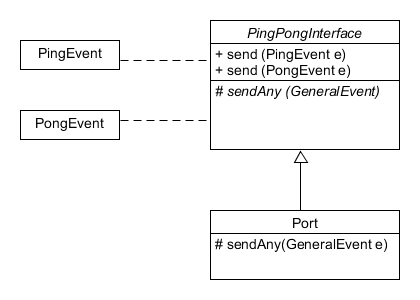
\includegraphics[scale=0.7]{inf_ver2.png} \\
Előnyök:
\begin{itemize}
\item Általános megoldás, az interfészt ténylegesen megvalósítjuk, így ez akár modell osztályokra is kiterjeszthető
\item Funkcionálisan nem különülnek el a \textit{send} függvények egymástól, így a karbantartási idő nem nő
\end{itemize}
Hátrányok:
\begin{itemize}
\item A generált kód mérete azonban jelentősen megnő, mivel több \textit{send} függvény generálásra van szükségünk, melyek csak a várt szignál típusban különböznek.
\end{itemize}
\item Mint a fentiekből látjuk, az utóbbi megoldásnak egy hátránya van, hogy növeljük az interfész kódját az első megoldáshoz képest. Amíg csak generáljuk az interfészt, addig ez elhanyagolható tényező, azonban, ha kézzel kell hozzáadni a programunkhoz, hogy kiterjesszük a modellel való kommunikációt, már probléma lehet. Megfigyelhetjük, hogy minden interfész implementációja csak abban fog különbözni, hogy különböző szignálokat tudnak fogadni. A C++ template metaprogramozási lehetőségeit kihasználva próbáljuk meg az interfész kódját egészen odáig szűkíteni, hogy csak fel kelljen sorolni egy típuslistába, hogy milyen szignálokat tud küldeni illetve fogadni. \\
Cél szintaxis: \textit{using PingPongInf = GeneralInterface<Ping,Pong>} \\
Ez azt jelentené, hogy a \textit{PingPongInf} egy olyan interfész lenne, amelynek két fogadó művelete van, a Ping és a Pong.\\
Vizsgáljuk meg a szolgáltatott részt, az elvárt ezzel analóg. Vezessünk be egy olyan sablon \textit{send} függvényt, melynek a sablon paramétere az elküldendő szignál típusa. Ezt látjuk a publikus interfészen, eszerint bármilyen szignállal meg tudjuk hívni az adott függvényt. Azonban a függvény delegálja a hívást egy olyan védett sablon függvénynek, mely bármilyen szignált képes fogadni,és rendelkezik egy logikai sablon paraméterrel: ebben adhatjuk meg, hogy a delegált szignál része-e az interfésznek vagy sem. 
Template specializáció segítségével kétféle implementációt adunk ennek a függvénynek: Az igaz ág, mely végrehajtja a szignál küldést, a hamis ág pedig szemantikai fordítási hibára fut, ezzel ellenőrizve fordítási időben, hogy ne adhassunk át olyan szignált, mely nem része az interfésznek. \\
A kérdés már csak az maradt, hogyan döntjük el egy adott szignálról, hogy része-e az interfésznek. Az egyik lehetőség bevezetni egy sablon osztályt, melynek egy adattagja megmondja, hogy reception szignálról beszélünk-e. Ezt alapértelmezetten hamisra állítani, és specializálni igaz értékekkel a sablon osztályt a megfelelő szignálokkal. \\
Összefoglalva az eddigieket egy ábrában: \\
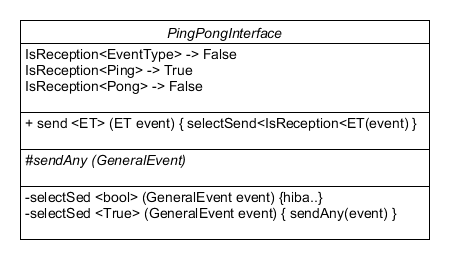
\includegraphics[scale=0.8]{better_inf.png} \\
Ezzel azonban még nem értük el a kívánt egyszerű szintaxist, de a \textit{send} függvényt legalább nem duplikáltuk fölöslegesen. A \textit{TYPELIST} \cite{typelist} konstrukciót használva viszont eljutunk a cél szintaxisig, ugyanis felsorolhatjuk a megfelelő szignál típusokat egy listába, és elég arra vizsgálnunk, hogy az adott szignál típus része-e a listának.
\end{enumerate}

A legutolsó megoldás tekinthető a legelőnyösebbnek, tartalmazza a második előnyeit, azonban a hátrányát sikerült kiküszöbölni.

\subsection{Szolgáltatott és elvárt interfészek megkülönböztetése}
\subsubsection{UML-ben}
Az UML szabvány szerint egy \textit{konnektor} csak olyan portok között
húzódhat, melynek a szolgáltatott és elvárt interfészei kompatibilisek egymással.
A port egy kommunikációs csomópontot reprezentál, a típusa azonban adattag révén tetszőleges lehet.
A modellosztály számára a port szolgáltatásokat nyújt a szolgáltatott interfész által, Így a típusa megfelel a szolgáltatott interfésznek.
A modellosztály azonban kifele áramoltathat a porton keresztül információkat, az elvárt interfész által.
Húzzunk be egy \textit{Using} reláció a port és az elvárt interfész között, mivel a modellosztály a portot használja üzenetáramoltatásra.
A probléma, hogy a \textit{Using} relációk nem kölcsönösen egyértelműek, ha két portnak ugyanaz a szolgáltatott interfésze, így
érdemes minden portnak egy saját interfészt generálni, amely leszármazottja a szolgáltatott interfésznek. Így minden port típusa egyedi lesz, és a relációk is egyértelműek lesznek a modellben.
\subsubsection{C++-ban}
Mivel a portra tudunk üzentet küldeni, de fogadni is tudunk róla, így az interfészeknek két részük lesz, az egyik a fogadó, a másik a küldő műveleteket definiálja. Attól függően, hogy az adott interfészt szolgáltatott vagy elvárt interfésznek definiáltuk, a megfelelő részből fog leszármazni az adott port. A másik lehetőség az lenne, ha nem bontjuk két részre az interfészt, helyette a receptiön függvényeknek egy plusz paramétere lenne, hogy kívülről vagy belülről küldünk-e üzentet. (Ahogy azt a \ref{message} bekezdésben felvezettük ) Azonban a portok esetén problémába ütköznénk, mert a validáció nem tudna különbséget tenni aközött, hogy egy portnak szolgáltatott vagy elvárt interfésze-e, melyet implementál. \\

\subsubsection{Interfész kiterjesztetett szintaxisa, konkrét példa portok esetén}
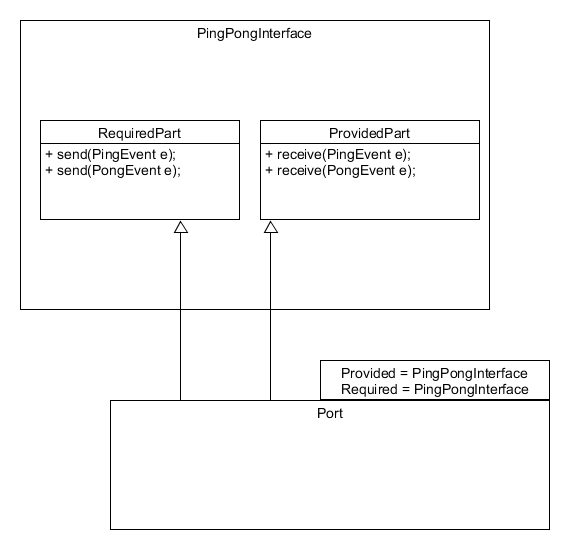
\includegraphics[scale=0.7]{seperate_inf.png} \\

\section{Konnektorok, összekapcsolás művelet reprezentálása} \label{connect}
Az interfészeket (\ref{inf}) és portokat már tudjuk exportálni UML-ben, illetve megfelelő C++ reprezentációt is találtunk. A konnektorokat ezek segítségével már ki tudjuk fejezni. \\
Mivel \textit{txtUML}-ben 1-1 kapcsolatokat tudunk csak leírni, így a mi megoldásainkat is erre korlátozzuk. Először megvizsgáljuk, mi lehet a szabványos reprezentáció UML-ben, majd kitérünk a különböző megoldásokra C++-ban. \\
Mielőtt még tovább megyünk, definiáljuk, pontosan mik ezek a konnektorok az UML szerint. A konnektorok alapvetően portokat kötnek össze, de többet fejez ki egy egyszerű asszociációnál. A konnektor egyfajta absztrakciót fejez ki két port között, leírja, milyen két port kapcsolódik össze, delegációval vagy assembly kapcsolattal vannak-e összekötve, illetve a kommunikáció prototípusát is képes leírni. A delegáció szülő-gyerek portok között jöhet lére, ilyenkor egy portra való üzenetküldést delegálunk a túloldalon lévő portra, mely tovább áramoltatja a belső komponens felé, vagy a másik irány esetén a külvilág felé, a komponensen kívülre. Assembly összekapcsolás esetén két egyenrangú enkapszuláció portja között jön létre kapcsolat, kölcsönös, oda-vissza kommunikációval. Fontos, hogy szülő-gyerek enkapszulációk között nem lehet Assembly kapcsolat, illetve egyenrangú szereplők között Delegáció.
\subsubsection{Konnektor reprezentáció UML-ben}
A szabvány szerinti reprezentáció viszonylag értelemszerű, egy \textit{Connector} UML elemet kell létre hozni, a végeknek megadni a portokat, beállítani, hogy Assembly vagy Delegált összekapcsolás van-e közöttük. A \textit{Connector} elemnek van egy Asszociáció típusa, mivel a szabvány szerint a \textit{Connector} egy Asszociáció egy konkrét realizációja. Hogy mi legyen ez a típus, azzal később foglalkozunk.

\subsubsection{Összekapcsolás művelet reprezentációja UML-ben}
A \textit{connect} akció kifejezése UML-ben már kevésbé egyértelmű, mivel \textit{connect} akció nem létezik explicit a szabványban. Több lehetőséget is megvizsgáltunk, mire eljutottunk a helyes reprezentációhoz.
\begin{enumerate}
\item Mivel a Portok adattagok az UML-ben (Property-k) így két portot kölcsönösen értékül adhatunk egymásnak. Ez egy lehetőség lehet kifejezni az összekapcsolást, szabványos modell keletkezik, de mégsem ez a helyes szabványa Portok összekapcsolásának. A probléma ugyanis az lesz, hogy bármilyen két portot összekapcsolhatok így, konkrét konnektor realizáció nélkül.
\item Mivel a \textit{Connector} egy asszociáció példány, így már egy konkrét, létrejött kapcsolatról beszélhetünk. Ebből adódóan a komponensek struktúrájából következtethetünk az összekapcsolt portokra. Azonban ez megszorításokkal járna, ha például egy szülőnek két azonos típusú gyereke van, de csak az egyikkel szeretne delegáció révén kommunikálni, nem köthetem hozzá mindkét gyerek porthoz a szülő portját. \\
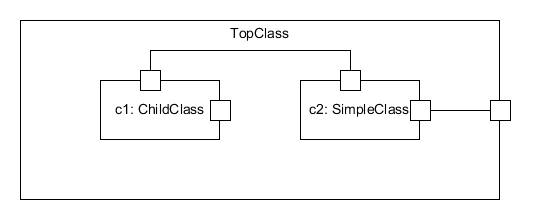
\includegraphics[scale=0.8]{preconnect_problem.png}
\item Nem maradt más lehetőség, mint a dinamikus összekapcsolás, és szintaktikailag sincs már más lehetőségem, mint a \textit{CreateLinkAction} használata, melyet a szabvány definíciója is sugall. Ehhez két dologra van szükségem: Végpontokra, valamint arra az asszociációra, melyet használni szeretnék az összekapcsoláshoz. Mint korábban láttuk, a Konnektorok fel vannak típusozva egy Asszociációval. Értelemszerű lenne ezt fölhasználni az összekapcsoláshoz, a kérdés csak az, mi legyen ez az Asszociáció. Az Asszociáció típusok között húzható, a Port önmagában nem típus, azonban adattag révén rendelkeznek típussal, a szolgáltatott interfészük típusával. Nem maradt más ésszerű lehetőségünk, mint ezek között az interfészek között létrehozni egy Asszociációt, melyet a Konnektor realizál a Portok összekapcsolásával. Így a \textit{CreateLinkAction}-be be tudjuk tenni Asszociációként a Konnektor típusát, ami mentén összekapcsolunk. Ezzel egy szabványos UML-t generálunk, és a Konnektorokat sem hagyjuk figyelmen kívül két port összekapcsolásánál. \\
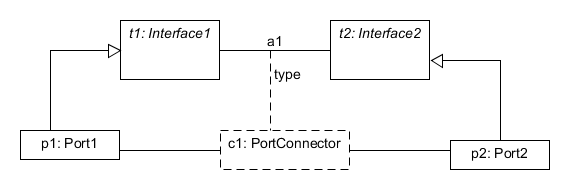
\includegraphics[scale=0.8]{connect_type.png}
\end{enumerate}

\subsection{Összekapcsolt portok reprezentációja C++-ban} \label{conn_cpp}
A szabvány szemantikája szerint, amikor egy üzenet küldünk a \textit{send} művelettel egy adott portra, annak továbbítania kell ezt a vele kapcsolatban álló port felé. Ehhez mindenképpen valami referenciát kell tárolni a kapcsolat Portra. Ezt alapvetően kétféle képen érhetük el:\\
\begin{enumerate}
\item Egy globális adatszerkezetben, példásul egy asszociatív tömbben megmondjuk, melyik porthoz ki kapcsolódik. Ennek előnye, hogy nem a Port kódja semleges marad, nem kell belekódolni a kapcsolatokhoz.
Hátránya az, hogy egy párhuzamos környezetben egy globális adatszerkezetet kell manipulálni, így sok szinkronizációt igényel a dolog, minek következtében csökken a hatékonyság
\item A másik lehetőségünk, hogy a port kódjában közvetlen referenciát tárolunk a kapcsolt portra. Mivel az nem lesz érdekes az üzenetküldés szemantikájában, hogy pontosan melyik Konnektoron keresztül kapcsolódnak az adott portok egymáshoz (annak típusa azonban számítani fog), és csak 1-1 kapcsolatok valósítunk meg, így a Port kódját nem kell a modell alapján generálnunk, nem fog bővülni, és hatékonyabb megoldást érhetünk el szekvenciális környezetben is, mint a globális adatszerkezettel. 
\end{enumerate}

Az üzenetküldés szemantikájához már megvan a referenciánk, azonban ez még nem elég önmagában. Figyelembe kell vennünk azt is, hogy milyen típusú Konnektoron keresztül kapcsolódtak az adott portok. Másképp kell átadni az üzenetet, ha Delegációról van szó, és másképp, ha Assembly kapcsolatról. Delegáció esetén, ha üzenetet küldünk kívülről egy adott portra (\textit{send} művelet), akkor a szemantika szerint az üzenetküldésünk ekvivalens a kapcsolt portra való belső üzenetküldéssel. Assembly kapcsolat esetén azonban ez az üzenetküldés a kapcsolt portra való külső üzenetküldéssel lesz ekvivalens a műveletünk. (\textit{receive} művelet). Így tudunk kell, hogy a referenciánk milyen kapcsolatban áll a portunkkal. Két lehetőségünk van ennek kifejezésére, a választás nem egyértelmű:
\begin{enumerate}
\item Virtualizáció használata, \textit{Port} referencia helyett \textit{Connection} referencia, melynek absztrakt művelet eldönti, a kapcsolt port melyik műveletét kell meghívni. Ez egy tisztább implementáció, azonban a virtualizáció nem elég hatékony. \\\\
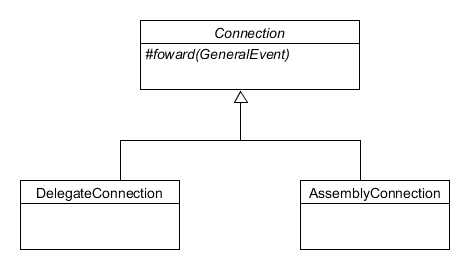
\includegraphics[scale=0.7]{connection.png} \\ \\
\item Delegáció jelző használata: Marad a Port referencia, maga a Port dönti el, melyik művelet hívására van szükség a jelző alapján. Ez a megoldás kevésbé letisztult, de hatékonyabb. \\

\end{enumerate}

Vizsgáljuk meg az üzenet fogadás szemantikáját is. A fogadás művelet végrehajtási szemantikája attól függ, hogy állapotgéppel összekapcsolt Portrol (Behavior Port) beszélünk-e vagy általános portról. Előbbi esetén egy objektum állapotgépéhez futnak be az üzenetek, a másik esetben pedig a szülő komponens portja delegálja az üzenetet a gyerek klasszifikáció portjára. Ennek megvalósítására szintén a fent említett két lehetőségünk van, a virtualizáció, illetve a behavior jelző. Egy \textit{Behavior Port} esetén nem csak a \textit{receive} művelet törzse különbözik, de más-más adattagokkal dolgozik a két port. Állapotgép összekapcsolás esetén referenciát kell szereznünk az állapotgépet birtokló objektumra, egyéb esetben pedig a gyerek komponens portjára. Ez különböző adattagokat igényel, az adat redundancia miatt leszármazás egy kézen fekvő választás. Unio típus segítségével azonban el lehetne kerülni a redundáns tárolást, ami egy hatékonyabb, de nehezebben olvasható kódot eredményez.
\\

\subsubsection{Különböző port típusok megvalósítása szemléltetve}
\begin{enumerate}
\item Leszármazással: \\\\
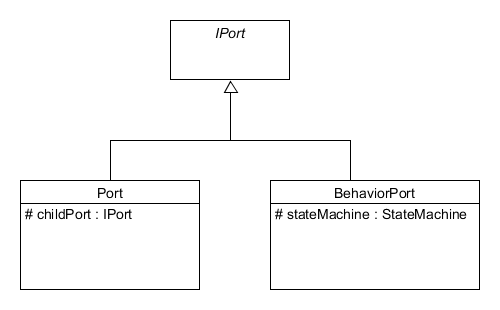
\includegraphics[scale=0.7]{behav_generalport_diag.png} \\

\item Behavior jelzéssel: \\
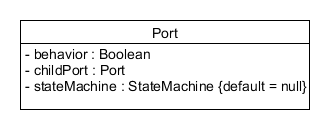
\includegraphics[scale=0.7]{simple_port_diag.png}

\item Unio típussal: \\
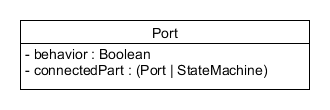
\includegraphics[scale=0.7]{unio_port_diag.png}
\end{enumerate}

Hasonlóan az interfészekhez, a kapcsolatok esetén is a kevert megoldás lenne a leghatékonyabb. Ha dolgozhatnánk leszármazással, ugyanakkor nem kéne virtualizációt használni. Erre egy kézenfekvő megoldás az lenne, ha a leszármazáskor megadnánk az interfésznek, ki a leszármazottja. \\
\textit{class DelegateConnection : public Connection}$<$\textit{DelegateConnection}$>$ \\
Majd definiálnánk a speciális implementációkat, az interfész implementáció pedig statikus konverzióval a specializált \textit{Connection} osztályra konvertálná önmagát, és meghívná a megfelelő műveletet. Ehhez fordítási időben tudnom kell, hogy egy adott porthoz milyen típusú kapcsolaton keresztül fog létrejönni a referencia. \\ 
A portokat akkor kapcsoljuk össze, mikor létre hozzuk a rendszer struktúráját. Minden port 1-1 kapcsolattal kapcsolódik egymáshoz. Ami azt jelenti, hogy egy állapotgéppel összekapcsolt port esetén egy referenciák lesz egy másik portra, melyet valamilyen ismert kapcsolaton keresztül kötünk majd hozzá. Általános port esetén pedig két referenciánk lesz, az egyik biztosan egy delegáció, a másik pedig ugyanazon az érvek mentén ismert, amit az előbb tárgyaltunk. Ebből következtetve úgy tűnik, hogy ha a pontos összekapcsolások nem is ismertek, a potenciális összekapcsolások típusai igen, így fordítási időben el tudjuk dönteni egy adott kapcsolatról, milyen típusú. Az is lehetséges, hogy egy félkész, vagy hibás modell exportálása esetén egyáltalán nem adunk meg Konnektort két port között. Ilyenkor exportálási hibát nem szeretnénk adni, mivel lehetséges, hogy a felhasználót tudatosan érdekel egy ilyen modellnek a C++ kódja, helyette inkább bevezetünk egy \textit{NoConnection} típusú leszármazást, melynek műveleteinek szemantikája megegyezik az üres utasítással. Akár sablon specializációval is dolgozhatunk, mely azért is lesz előnyös, mert megspórolhatjuk a benne eltárolt port referenciát.

\subsubsection{Megoldás szemléltetése}
\begin{enumerate}
\item \textit{NoConnection} leszármazással: \\
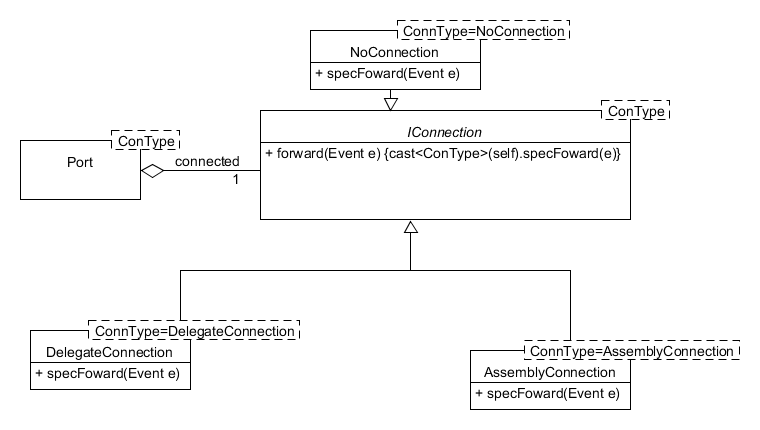
\includegraphics[scale=0.6]{extended_connection.png}
\item \textit{NoConnection} specliazizációval: \\

\end{enumerate}

\subsection{Konnektorok reprezentálása C++-ban}
A konnektorok reprezentálása is több lehetőségünk van, ezeket fogjuk most megvizsgálni
\begin{enumerate}
\item Itt is felmerül a lehetőség, hogy teljesen figyelmen kívül hagyjuk a konnektorokat. Ezt akkor tehetjük meg egyértelműen, ha a referencia birtoklását választjuk a fentiekben az összekapcsolt portok reprezentálásánál. Ennek előnye szintén az egyerűség lesz, a generált kód mérete kisebb lesz. Hátránya pedig a validáció teljes hiánya. Az interfészeknél arra jutottunk, hogy szükséges a validáció, így ez nem a legjobb megoldás.
\item A másik lehetősünk bevezetni egy \textit{Connector} osztályt, és összekapcsolásánál erre az osztályra hivatkozunk. Ebben a struktúrában leírhatnánk a portokat, melyek potenciálisan kapcsolódnak egymáshoz, és ezt használhatjuk validációra. Ennek előnye egy tiszta reprezentáció lesz, hátránya viszont az, hogy egy redundáns megoldást kapunk, a konnektoroknak semmi szerepük nincsen a validáción kívül.
\item A Konnektorokhoz generált asszociáció típust használjuk fel a validációra. Ennek előnye, hogy az asszociációkat egyébként is eltengethetetlen generálunk a modellben, így nem igényel további kódgenerálást. Azonban a típusvalidációról gondoskodik, nem enged összekapcsolni olyan két portot, melyhez nem tartozik megfelelő típusú asszociáció. Hátránya, hogy nem elég konkrét, nem kell megfelelni a konkrét portoknak a struktúrán belül, elég, ha az interfészeik megfelelnek.
\item A legoptimálisabb megoldás most is a két megoldás előnyeinek az összekeveréséből lesz. A \ref{conn_cpp} fejezetben megállapítottuk, hogy fordítási időben képesek vagyunk eldönteni egy adott portról, hogy az milyen típusú kapcsolatban állhat a referenciában lévő porttal. Ez azért van, mert ismerjük a modellből a Konnektor struktúrákat, és egyértelműen el tudjuk dönteni, potenciálisan milyen kapcsolat jöhet létre a két port között. Ha nem tudnák eldönteni, egy redundáns, hibás modellt írtunk, mellyel most nem foglalkozunk. Ennél fogva, a konnektorból nem csak annak típusát, de azt a szerep nevet is ki tudjuk nyerni, mely meg fog egyezni a generált asszociáció szerepneveivel. A \textit{Connection} referencia típusában pedig nem csak azt kódolhatjuk bele, milyen típusú kapcsolatban áll az adott porttal, hanem azt is, hogy az átellenes port milyen szereppel van jelen. A referenciák beállítása pedig csak egy olyan típusú \textit{Connectiont} enged beállítani, ami megfelel a szerep típusúnak. A szerepeket a port sablonparaméterében adhatjuk meg. Ha egy hiányos modellben nincs kapcsolatban egy port egy adott \textit{Connector}-on keresztül egyetlen másikkal sem, akkor megadhatnánk egy extremális \textit{NoRole} szerepet, de itt már egyértelműen érdemes sablon specializációval dolgozni, és a \ref{conn_cpp} fejezetben említett módon egyszerűen használni a \textit{NoConnection}-re specializált verziót.  \\
Előnyök:
\begin{itemize}
\item Továbbra is elég csak asszociációkat generálni a megfelelő szerepekkel.
\item A típus és szerep validációról is gondoskodunk, nem engedünk két olyan portot összekapcsolni, melyek között nincsen \textit{Connector}
\end{itemize}
Hátrányok:
\begin{itemize}
\item Azonban a portok kódja elbonyolódik sablonparaméterekkel, mely külső kód esetén nem optimális.
\end{itemize}
\end{enumerate}

\section{Kommunikáció megvalósítása C++-ban}
Végül még érdemes néhány szót ejteni a kommunikációs szemantikáról. Ennek nagy részét már tisztáztuk. Megvizsgáltuk a portra való üzenetküldés szemantikát az enkapszuláción belülről. Ekkor az üzentet kifele áramoltatjuk, egy másik port fogja megkapni. Ebben a fejezetben csak az lesz az érdekes, hogy az üzenetáram végén, amikor eljut az üzenet egy állapotgéphez, hogyan fogjuk kezelni. Így csak az állapotgéppel összekapcsolt portok fogadó (\textit{receive}) műveletei lesznek érdekesek számunkra. A port tartalmaz egy referenciát az állapotgépre, így tudja neki továbbítani az üzenetet. Azonban a nyers továbbítás kevés lenne, mivel egy objektum állapotgépe egy adott porton történő állapotváltozásra kell reagáljon. Így az üzenet feldolgozásakor tisztában kell lennünk azzal, melyik porttól kaptuk meg az adott üzenetet. Az UML szabványban egy adott átmenetnél felsorolhatjuk az adott portokat, melyről az adott üzenetet várjuk. \textit{txtUML}-ben csak egy portot adhatunk meg, vagy jelezhetjük, hogy az adott üzenet bárhonnan érkezhet, porton kívülről is, vagy bármely portról. Ennek megfelelően megfelelően mindenképpen a meglévő állapot-átmenet táblát érdemes kibővíteni egy új dimenzióval: Megadni, hogy az átmenetben szereplő üzenet potenciálisan mely portokról jöhet, hogy az állapotgép reagáljon rá. \\
Eddig esemény-állapot táblánk volt, mely megadta, melyik átmenetnek kell végrehajtódnia. Ezt kibővíthetjük az alábbi módokon:
\begin{enumerate}
\item Egy darab port típus, és állapot-esemény-port hármasokat fog tartalmazni az átmenet táblánk. Mielőtt egy port továbbítja az állapotgépnek az üzenetet, beállítja az eseményen a port infót, így tudni fogjuk, honnan érkezett. Ez az esetünkben jól fog működni, mivel csak egyféle portról jöhet az üzenet. Azonban, ha azt adjuk meg, hogy bármelyik portról érkezhet az üzenet, már problémákba ütközünk, mivel ilyenkor nincs megadva port dimenzió a táblában, az üzenetben viszont igen. Ezt speciálisan le tudjuk kezelni az üzenetfeldolgozás során, azonban ez nem elég általános megoldás. \\

\begin{center}
\begin{tabular}{@{}ccc|c@{}} \toprule
\multicolumn{4}{c}{Átmenet tábla} \\\midrule
Esemény & Állapot 	& Port 	& Átmenet-Őrfeltétel\\\midrule
Event1 	& State1 	& Port1 & Ttransition1-Guard1 \\
... 	& ... 		& ... 	& ... \\
EventN 	& StateN 	& PortN & TtransitionN-GuardN
\end{tabular}
\small
\end{center}
\item Általánosabb megoldás, ha a port helyett megadhatnánk egy maskban azokat a portokat, melyek üzeneteit megfigyeli az adott átmenet. Mivel egy üzenet továbbra is csak egy helyről érkezhet, így elég lenne csak azt vizsgálunk, hogy az állapot-esemény alapján megkeresett átmenet portjai között szerepel-e a az a port, melyről az üzenet érkezett. Fontos, hogy itt a Port dimenzió a táblázat másik végén jelenik meg. A táblából, hasonlóan az eddigiekhez, állapot-esemény pár alapján keresünk, melyből megkapjuk az átmenet függvénymutatót, az őrfeltételt, valamint a megfigyelt portokat. Ekkor azt az átmenetet hajtjuk végre, melynek portjai között szerepel az üzenet portja vagy a \textit{NoPort} speciális típus. \textit{AnyPort} esetén az összes lehetséges Portot belerakjuk az átmenetbe, valamint a \textit{NoPort} típust is. \\

\begin{center}
\begin{tabular}{@{}cc|c@{}} \toprule
\multicolumn{3}{c}{Átmenet tábla} \\\midrule
Esemény & Állapot 	&  Átmenet-Őrfeltétel-Portok\\\midrule
Event1 	& State1 	&  Ttransition1-Guard1-Ports1 \\
... 	& ... 	 	& ... \\
EventN 	& StateN 	& Ttransition1-Guard1-PortsN
\end{tabular}
\small
\end{center}
\end{enumerate}

\chapter{Program dokumentáció}
A dolgozatban nem csak elemeztük a lehetséges megoldásokat, hanem kiválasztottunk egy lehetséges megoldást, melyet leprogramozva demonstrálni tudjuk a dolgozat eredményeit. A továbbiakban ennek a demonstrációs programnak a rövid felhasználói és fejlesztői dokumentációja következik.

\section{Felhasználói dokumentáció}
A dolgozat a \textit{txtUML} keretrendszerre épül, melynek részletes felhasználói dokumentációja megtalálható az alábbi linken: \url{http://txtuml.inf.elte.hu/wiki/doku.php}

A dolgozat szempontjából a Portok, Interfészek, Konnektorok leírása a legfontosabb, valamint az exportálás és fordítás.

\subsection{Szükséges eszközök}
Az exportáláshoz az alábbi eszközökre van szükség:
\begin{itemize}
\item Java
\item Eclipse IDE az export dialog eléréshez, minden szükséges függőség letöltődik a txtUML pluginnal
\end{itemize}

A fordításhoz az alábbiakra van szükségünk
\begin{itemize}
\item Cmake segítségével legenerálhatjuk a számunkra tetsző fordítási környezetet
\item GCC vagy Clang
\item A generálandó fordítási környezet. (MinGW, Ninja, MSVC, stb..)
\end{itemize}

\subsection{Generálás és futtatás}
Kódot generálni legegyszerűbben Eclipse-ből tudunk egy txtUML modell megírása és egy kihelyezési konfiguráció alapján. A \textit{runtime} mappában az előre megírt fájlokat másoljuk, mely tartalmazza többek között a Portok osztályát is, az összekacsoló műveleteket, és azok szemantikáját. A konkrét port példányokat, konnektorokat, interfészeket pedig a \textit{runtime} mappán kívül generáljuk a modell alapján. \\

A generált kódot fordítani a \textit{cmake}, valamint a választott build környzet parancsával tudunk. A \textit{cmake} parancs elhagyható, ha az exporter dialóguson kiválasztjuk a megfelelő környezetet. Fordítás után pedig már futtathatjuk a \textit{main} futtatható állományunkat.

\section{Fejlesztői dokumentáció}
A program a \textit{txtUML} keretrendszer C++ fordító és exporter komponensét fejleszti tovább, ennél fogja Java nyelven készült. A Java modellt JDT segítségével járjuk be, és az EMF keretrendszert használjuk a szabványos modell létrehozásához. \\

\subsection{Szerkezeti felépítés}
A program négy jól elkülöníthető részből áll, mindhárom részt ki kellett egészíteni a Portok, Interfészek, Konnektorok exportáláshoz

\begin{enumerate}
\item A Java modellt UML modellre leképző algoritmusok. Ezek nem tiszta Java-ban, hanem a Xtend keretrendszerben készültek. A strukturális elemekhez fel kellett venni a \textbf{PortExporter.xtend}, \textbf{InterfaceExporter.xtend}, \textbf{ConnectorExorter.xtend} és a \textbf{ConnectorEndExporter.xtend} fájlokat. Az akcióelemekhez pedig felvettük a port referenciát kiolvasó \textbf{PortReferenceExporter.xtend} fájt, az üzenetküldéshez a \textbf{SendToPortActionExporter.xtend}, az összekapcsolásokhoz a \textbf{AssemblyConnect.xtend} valamint a \textbf{DelegateConnect.xtend} fájlokat.
\item Az UML modellt feldolgozó algoritmusok. Itt hozzá kellett adni a  \textbf{PortExporter.java} és az \textbf{InterfaceExporter.java} osztályokat, melyek ezek struktúrájának az exportálásáért felelnek. A \textit{send} és a \textit{connect} műveletek exportálása végett hozzá kellett nyúlni az \textbf{ActivityExporter.java} osztályhoz, mely az akciókódok exportálásáért felelős.
\item C++ kódgenerálási sablonok: Itt bevezettük a \textbf{InterfaceTemplates.java} és \textbf{PortTemplates.java} fájlokat a strukturális elemek sablonjához. Az \textbf{AssociationTemplates.java} az összekapcsoláshoz szükséges sablonokról gondoskodik.
\item Előre megírt C++ fájlok: Itt lényegében a \textbf{PortUtils.hpp} fájl tartalmaz minden portokhoz szükséges előre megírt elemet: A portok típusát, a kapcsolatokat, az összekapcsolásokat. Az \textbf{IEvent.hpp}-be is bele kellett nyúlni az eseményfeldolgozás megváltozása miatt. Valamint az \textbf{InterfaceUtils.hpp} tartalmazza az interfészek sablonját és az üres interfészt, a \textbf{AssociationUtils.hpp} pedig az összekapcsoláshoz szükséges asszociációk sablonját.
\end{enumerate}

Ezek a modulok jól eltönkretehetőek és cserélhetőek. 

\subsection{Tesztelés}
A demonstrációs program néhány tesztesetét szedjük össze az alábbi fejezetben.

\begin{enumerate}
\item Regresszió tesztelése: Portok nélküli modell létrehozása, melyben azt várjuk, hogy az eredmény maradjon az, ami eddig volt.
\item Egyosztályos modell létrehozása egy darab porttal
\begin{enumerate}
\item Üres interfészekkel, \textit{send} művelet kipróbálása, mely hibás lesz
\item Nem-üres interfésszel, \textit{send} művelet kipróbálása olyan szignállal, melyet tartalmaz az interfész. Nincs fordítási hiba, de nincs hatása sem. Majd egy olyannal, mely nem része az interfésznek.
\item Nem-üres interfésszel, állapotgéppel összekapcsolt portot hozunk létre. Az osztály egy átmenete tartalmazza az adott portot. \textit{receive} művelet kipróbálása.
\end{enumerate}
\item Kétosztályos modell létrehozása, egy szülő osztály, melynek van egy belső osztálya. Mindkettőnek van egy-egy portja.
\begin{enumerate}
\item Kompatibilis interfészekkel hozzuk létre őket, delegációval összekapcsoljuk őket, majd \textit{send} művelet kipróbálása a belső komponensen. Ezután a \textit{receive} művelet a külső komponensen.
\item Assembly kapcsolattal összekapcsoljuk őket, mely fordítási hibát jelez.
\item Inkompatibilis interfészekkel hozzuk létre őket, majd delegációval megpróbáljuk összekapcsolni, mely szintén fordítási hibát jelez.
\end{enumerate}
\item Komplex modell létrehozása, mely demonstrációs célokra is megfelelő: Egy ping-pong játék struktúra létrehozása, mely tartalmaz egy táblát, valamint egy bírót. Ezek tartalmaznak egy-egy portot, melyek Assembly kapcsolattal vannak összekötve. A tábla tartalmaz két játékost, melyek két portot tartalmaznak, egy ping-pong portot, valamint egy olyan portot, melyről a játék kezdése üzenetet várják. A ping-pong portok egymással vannak összekötve, ezen keresztül passzolgatnak egy szignált oda-vissza a játékosok egymás közt, az első játékos pedig delegációval hozzá van kötve a táblához. A játék indulásakor a bíró lead egy játék kezdése szignált a táblának, melyet tovább delegálunk a kezdő játékosnak, és ő elindítja az első szerválást.
\end{enumerate}

A generált kódok megfelelőek, a modellek pedig az elvárt működésnek megfelelően működnek.

\begin{thebibliography}{4}


\bibitem{uml_omg}
	OMG, Superstructure
	\emph{Unified Modeling Language (OMG UML)}

\bibitem{uml_real}
	Bran Selic, ObjecTime Limited
	Jim Rumbaugh, Rational Software Corporation
	\emph{Using UML for Modeling Complex Real-Time Systems}
	\url{ftp://ftp.omg.org/pub/umlrtf/UML_rt_ext_F56dist.pdf}
	

\bibitem{txtUML}
  Gábor Ferenc Kovács, Ádám Ancsin, Gergely Dévai,
  \emph{Textual, executable, translatable UML},
  14th International Workshop on OCL and Textual Modeling, 
  2014. 

\bibitem{alf}
	Object Management Group. 	
	\emph{Action Language for Foundational UML (ALF), standard, version 1.0.1.}
	\url{http://www.omg.org/spec/ALF/} 2013
\bibitem{fmul}
	Object Management Group. 
	\emph{Semantics of a Foundational Subset for Executable UML Models (fUML), standard, version 1.1}
	\url{http://www.omg.org/spec/FUML/1.1/} 2013
	
\bibitem{umple}
	Andrew Forward, Omar Badreddin, and Timothy C Lethbridge
	\emph{Umple: Towards combining model driven with prototype driven system development}
	In Rapid System Prototyping (RSP), 2010 21st IEEE International Symposium on, pages 1–7. IEEE, 2010.

\bibitem{bridge}
	OneFact.	
	\emph{BridgePoint xtUML tool.} 
	\url{http://onefact.net}
	
\bibitem{startuml}
	StartUML Tool
	\url{http://staruml.io/}
	
\bibitem{typelist}
	TypeLists and a TypeList Toolbox via Variadic Templates
	\url{https://www.codeproject.com/Articles/1077852/TypeLists-and-a-TypeList-Toolbox-via-Variadic-Temp}

	
\end{thebibliography}

\end{document}
